%%%%%%%%%%%%%%%%%%%%%%%%%%%%%%%%%%%%%%%%%%%%%%%%%%%%%%%%%%%%%%%%%%%%%%%%%%%
% Copyright (c) 2010 committers of YAKINDU and others.
% All rights reserved. This program and the accompanying materials
% are made available under the terms of the Eclipse Public License v1.0
% which accompanies this distribution, and is available at
% http://www.eclipse.org/legal/epl-v10.html
%
% Contributors:
%     committers of YAKINDU - initial API and implementation
%%%%%%%%%%%%%%%%%%%%%%%%%%%%%%%%%%%%%%%%%%%%%%%%%%%%%%%%%%%%%%%%%%%%%%%%%%%
\section{Setting Up The Example Project}

The reference example used within this documentation is the \emph{TrafficLight}
example project deployed with the YAKINDU distribution. To set it up in your
local workspace, use the YAKINDU Example Project Wizard as depicted by Figures
\ref{fig:screenshot1} and \ref{fig:screenshot2}. 
\begin{figure}[h!] 
\center
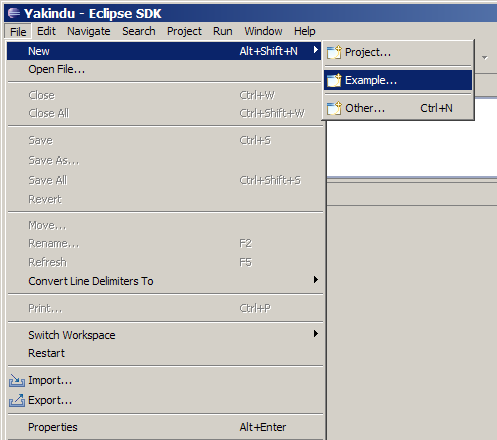
\includegraphics[width=0.5\textwidth]{./Pictures/Screenshot1}
\caption{\label{fig:screenshot1} Opening the Example Creation Wizard}
\end{figure}

\begin{figure}[h!]
\center
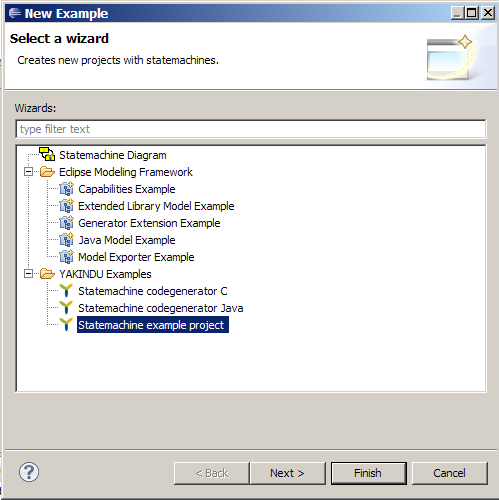
\includegraphics[width=0.5\textwidth]{./Pictures/Screenshot2}
\caption{\label{fig:screenshot2} Creating Statechart Example Projects}
\end{figure}

After successful completion, the Example Project Wizard will create the YAKINDU
Statechart example projects within the workspace, out of which one -
\emph{TrafficLight} - will serve as demonstration example in the following. As
outlined within Figure \ref{fig:screenshot3}, it denotes a state chart to control
a simple traffic light with a corresponding pedestrian light.

\begin{figure}[h!]
\center
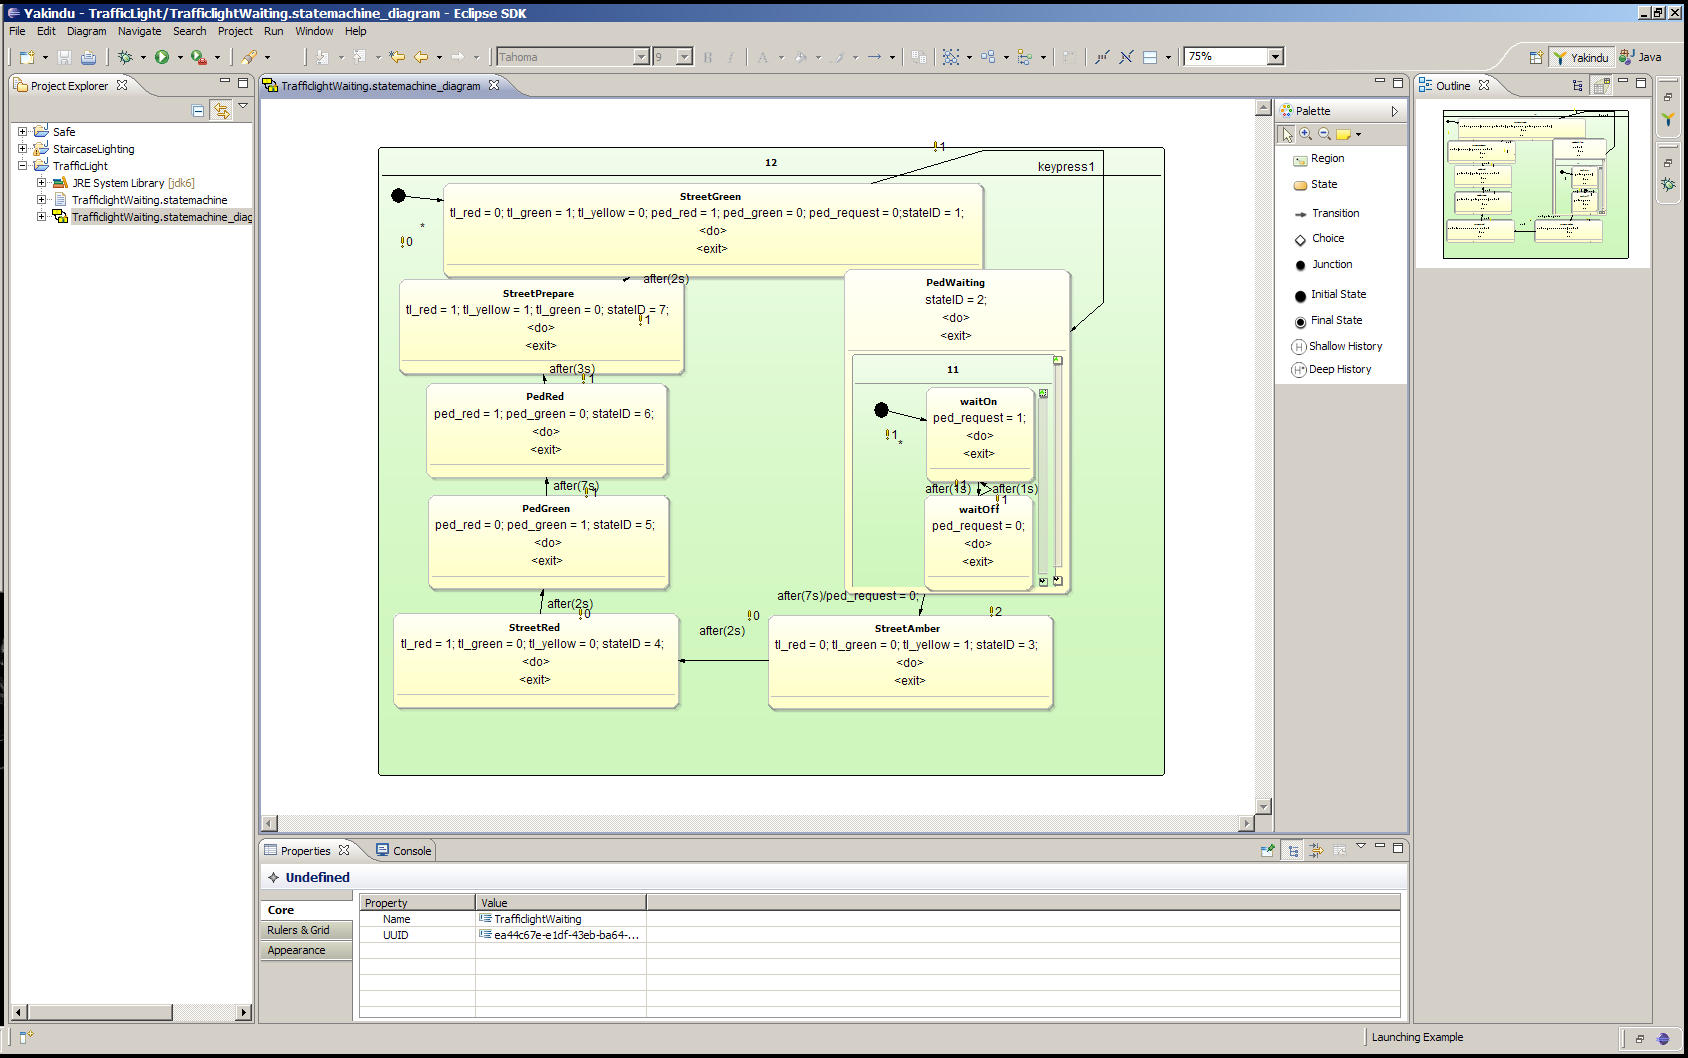
\includegraphics[width=\textwidth]{./Pictures/Screenshot3}
\caption{\label{fig:screenshot3} Traffic Light Example Project Contents}
\end{figure}

\clearpage